% !TeX spellcheck = en_GB
\section{Results (outline)}

\subsection{Validating the laser modules}

For every laser in the setup (561 nm, 640 nm, and 775 nm), I measured the polarisation state of the light at different points in the beam path and at the sample plane, by measuring the power transmitted by a linearly polarising filter at different angles relative to the beam. At the sample location, the 640 nm beam is quite well-polarised when set to a linear polarisation. When rotating a polariser, the transmitted power drops to about one fifth of the maximum. At the circular setting, though, the light is quite elliptical, with a minimum power transmitted through the polariser being about half as bright as the maximum, see \autoref{fig:640 laser pol at sample}. The quality of the 561 nm polarisation is higher. When set to a linear polarisation, the power transmitted through a polariser drop from about \SI{25}{\micro W} to a value almost equal to background levels around \SI{0.1}{\micro W}, while the amplitude variations of the circularly polarised light are withing 14\% of the mean, see \autoref{fig:561 laser pol at sample}. In conventional STED, the depletion beam is circularly polarised in order to achieve polarisation-independent quenching, so I also measured its polarisation state, see \autoref{fig:775 laser pol at sample}. The minimum power transmitted is about 63\% of the max. \todo{Calculate ellipticity angle, or introduce the $ E_{max}/E_{min} $ characteristic in the beginning.} \todo{Put this stuff into a table?}

There are two other things we can take away from those figures: the power of the 640 nm laser is not very constant. This can be explained by a slow ramp up to the set power every time the laser is turned on. Secondly, the noise on the signal from the 640 laser is higher. I believe this is due to the same effect. Therefore, I also measured the power profiles of the different lasers, see \todo{figure}. The conclusion from those measurements is that the response of the lasers to the desired power set in software is not linear at low powers. If experiments need to be done at low power, a neutral density filter is required. This is luckily not the case for biological specimens with a low density of fluorophores.

Finally, we also measured the PSFs of the different lasers as a sanity check. This is shown in \autoref{fig:normal psfs}. This data looks good. \todo{Why does it look good?} \todo{Mention how we got this data: PMT and gold beads.}

\subsection{Validating the detection module}

First off, I checked the polarisation dependence of the APDs. To do so, I ensured the light coming into the APDs was unpolarised by illuminating a sample of TetraSpec beads with circularly polarised 561 nm light, since that was the closest to circular that we could get. Then I put a polarising filter after the detection waveplates and measured the signal from the APD as a function of the incoming polarisation, see \autoref{fig:apd pol sensitivity}. For both APDs, there is a difference of about 4\%.

\textcolor{orange}{
To do:
	\begin{itemize}
		\item Should I do min/max like before? That would also be closer to a G factor, I guess.
		\item APD2 and power meter pol sensitivity.
		\item Correct for ellipticity of 561 polarisation
	\end{itemize}
} 

Second, I tested the effect of the detection waveplates on the polarisation state of incoming light. Linearly polarised input light was achieved by putting a polariser (P1) in the sample location and illuminating it with the microscope's top lamp. Then the intensity was measured by the APDs, which was dependent on the angle of a polariser located after the last waveplate (P2). Using Jones calculus, we know that two QWPs and a HWP can form a proper polarisation rotator \todo{ref methods}, but the default calibration (a function that maps the total rotation angle to the angles the waveplates have to take on) is unable to do so. I determined that a better calibration sets the (non-fixed) QWP to an angle of 50° and the HWP to half the rotation angle. The angle of the QWP was chosen such that it is aligned with the fixed QWP at the microscope end. The behaviour of both calibrations is shown in \autoref{fig:detection waveplate calibrations}. The new calibration works as expected.

\begin{figure}
	\centering
	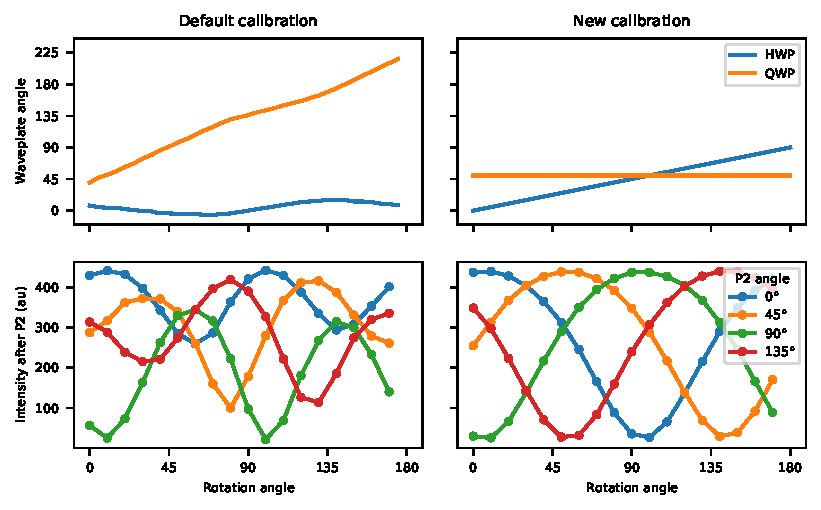
\includegraphics{detection waveplate calibrations.pdf}
	\caption{text}
	\label{fig:detection waveplate calibrations}
\end{figure}

Finally, I also measured the polarisation characteristics of the POL cube. I generated linearly polarised light as in the previous paragraph, but left out P2. Then I rotated the polarisation using the detection waveplates and measured the intensity of light reflected and transmitted by the POL cube into APD1 and APD2 respectively. Apparently, the degree to which the POL cube can split the signal is strongly dependent on the polarisation of the light at the sample (the angle of P1), \autoref{fig:pol cube effects}. The cause of this effect is not immediately obvious, but is most likely due to some birefringence present in the POL cube. \todo{Is that true?}

\begin{figure}
	\centering
	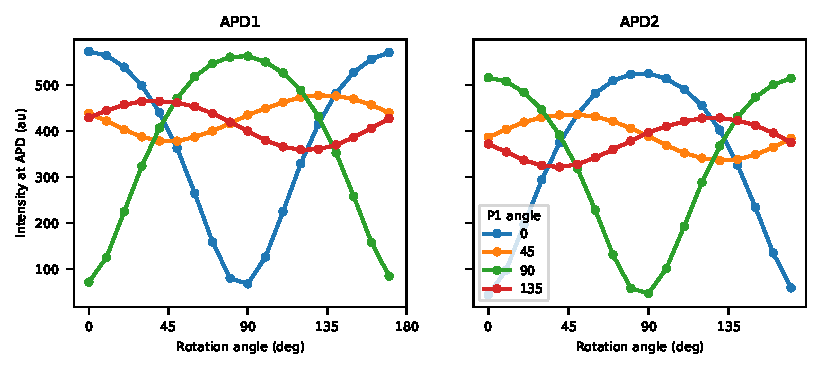
\includegraphics{pol cube effects.pdf}
	\caption{The POL cube distorts the polarisation state of incoming light. APD should measure the vertical component of the light (reflected by the POL cube), and APD2 should measure the horizontal component (transmitted). The detection waveplates were used to rotate incoming light, which was polarised along an angle shown in the legend.}
	\label{fig:pol cube effects}
\end{figure}

\subsection{Demonstration of conventional polarisation microscopy}

\begin{figure}
	\centering
	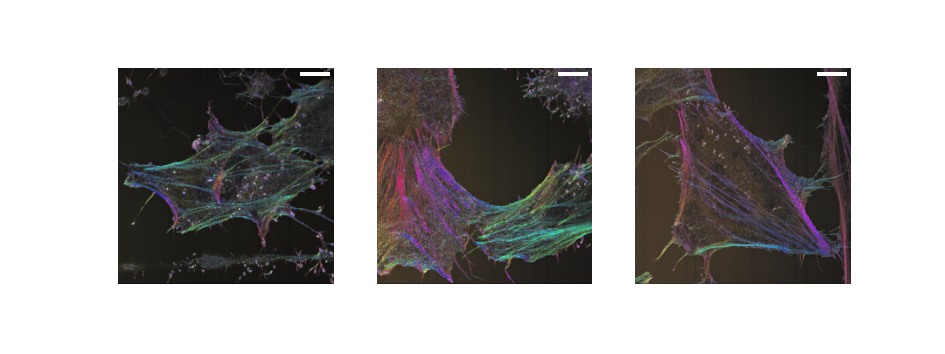
\includegraphics{conventional pol.pdf}
	\caption{
		Polarisation microscopy images of three different cells. Scale bars \SI{10}{\mu m}.
	}
\end{figure}

\textcolor{orange}{
	To do:
	\begin{itemize}
		\item Colour wheels in the images
		\item sSTED + polarisation
		\item Can I get some quantitative results?
	\end{itemize}
} 

\subsection{Polarisation-resolved STED microscopy}

\begin{itemize}
	\item Aligning the QWP
	\item Finding the HWP zero point
	\item Measuring the pSTED PSFs
	\begin{itemize}
		\item Power dependency on polarisation
		\item PSF orientation rotates with polarisation
	\end{itemize}
\end{itemize}





























